\chapter{Estado del Arte}\label{chap:estado_del_arte}


\indent Los algoritmos de sustracción de fondo (``\textit{Background Subtraction Algorithms}'') modelan esencialmente el segundo plano (``\textit{Background}'') de una imagen con la finalidad de detectar movimiento de objetos (''\textit{Foreground}'') en una secuencia de video. Aplicaciones como vigilancia a través de video, detección de movimiento y clasificación de acciones, necesitan primero modelar la imagen de fondo y luego detectar los objetos móviles.

\indent Modelar el fondo de imagen plantea una serie de desafíos que han sido abordados desde diferentes perspectivas por los investigadores. Cambios de luminosidad, movimientos simultáneos, ambigüedad (imprecisión) sombra y fondo, entre otros, constituyen parte de los problemas que deben superar los algoritmos de sustracción de fondo para detectar y clasificar eventos en una secuencia de imágenes. Se han elaborado en la comunidad variados conjunto de datos (``\textit{Datasets}'') \cite{singh_muhavi_2010, weinland_free_2006, schuldt_recognizing_2004, gross_cmu_2001, gorelick_actions_2007} que emulan escenarios y condiciones con el objetivo de evaluar robustez, rendimiento, calidad en clasificación, de los diferentes modelos de fondo desarrollados. Esta lista de escenarios, es un conjunto de situaciones generales normalmente encontradas en secuencias de video, las cuales constituyen un punto de comparación y referencia entre los diferentes algoritmos implementados en la comunidad. Una descripción más detallada de estas situaciones generales es mencionada en \cite{toyama_wallflower_1999}.

\indent Numerosos métodos de modelado de fondo han sido construidos considerando estas diferentes condiciones. Un estudio publicado por \textit{Bouwmans}\cite{bouwmans_recent_2011} (2011)  presenta un cuadro general de estos métodos y hace una clasificación en diferentes categorías dependiendo de la forma de construir el modelo del fondo. Un modelo básico consiste en usar promedios, medianas o análisis de histogramas en el tiempo. Una técnica simple es calcular el promedio de una escena sin objetos en movimientos, restar nuevos cuadros de esta imagen y comparar a través de un umbral. Otro tipo de modelo se construye basado en distribuciones estadísticas, particularmente en distribuciones del tipo ``\textit{Gaussianas}'', usando variables estadísticas para clasificar los píxeles. Se construyen modelos con redes neuronales en la que una red entrenada podría distinguir entre un píxel perteneciente al fondo o al objeto en movimiento. Otros modelos emplean ``\textit{clusters}'' para agrupar píxeles en diferentes elementos dentro de una secuencia. También existen modelos que emplean filtros especiales para hacer una estimación del fondo, como filtros de ``\textit{Kalman}'' o ``\textit{Tchebychev}''.  

\textit{Bouwmans}\cite{bouwmans_recent_2011} también evidencia un principio de funcionamiento de la mayoría de los métodos de sustracción de fondo, independiente del tipo de modelo e implementación usado. Establece ciertas etapas que se cumplen en los modelos de fondo: modelado de fondo, inicialización del fondo, mantenimiento del fondo, detección (\textit{foreground}), elección de medida de la característica (píxel, block, cluster), elección del tipo de característica (color, borde, texturas).

\section{Modelo de Mixtura de Gaussianas}

\indent Mixtura de Gaussianas (\textit{Gaussian Mixture Model - GMM}) ha sido uno de los métodos más mencionados en la literatura como herramienta de modelo estadístico para obtener el fondo de una secuencia de imágenes. Mixturas finita\cite{mclachlan_finite_2000} de distribuciones es una herramienta de modelado estadístico, análisis de datos e inferencias, usado como base para proporcionar modelos descriptivos de distribuciones en distintas áreas de aplicaciones. Tiene la propiedad (entre otras) de estimar parámetros en un esquema de aprendizaje no-supervisado, de observaciones producidas por un conjunto de fuentes aleatorias. En métodos de sustracción de fondo se utiliza mixtura de Gaussianas para modelar en el tiempo los valores de un píxel (o un vector de valores en espacio de colores RGB) y clasificar en diferentes categorías, generando ``\textit{clusters}'' de píxeles los cuales representan las diferentes mixturas de componentes.
 
\indent Uno de los primeros trabajos realizados con distribuciones estadísticas, que marca el inicio de investigaciones relacionadas con la utilización de mixtura de distribuciones para modelar fondo, es el trabajo de \textit{Friedman} y \textit{Russell} \cite{friedman_image_1997}. Ellos proponen, en un sistema de vigilancia del tráfico automovilístico, obtener el fondo mediante una composición fija de distribuciones Gaussianas. Modelan el valor de intensidad de un píxel con tres distribuciones predeterminadas, asociadas a tres diferentes tipos de objetos: vehículos, sombras, y camino (fondo de la imagen). Utilizan una versión incremental del algoritmo esperanza-maximización\cite{dempster_maximum_1977} (\textit{EM}), para inicializar y actualizar (como mecanismo de aprendizaje no-supervisado) los parámetros de la mixtura del modelo. La clasificación de píxeles es realizada comparando varianza con un umbral definido por la distancia \textit{Mahalanobis}. Durante el proceso de inicialización las tres distribuciones son etiquetadas por una heurística que determina como sombra el componente más oscuro, la distribución de vehículos se relaciona con una mayor varianza, y la distribución del camino con la menor varianza. 

Una aproximación similar es el trabajo de \textit{Stauffer} y \textit{Grimson}\cite{stauffer_adaptive_1999}. Ellos modelan el valor de un píxel con una mixtura de Gaussianas, a diferencia de \textit{Friedman} y \textit{Russell}\cite{friedman_image_1997} que utilizan un conjunto predeterminado de distribuciones para modelar un píxel. Ellos señalan que modelar el fondo mediante un conjunto fijo de distribuciones Gaussianas, el funcionamiento del sistema podría funcionar incorrectamente, con los píxeles que no estén  dentro de las distribuciones prefijadas. En su propuesta plantean, que la persistencia y la varianza de cada Gaussiana en la mixtura, determina las distribuciones que pueden corresponder a la imagen de fondo. Los píxeles que no se ajustan con las Gaussianas del fondo, se consideran parte de elementos en movimiento (\textit{Foreground}) y sólo son parte de éste, cuando existe consistente evidencia para convertirla en una nueva Gaussiana de las mixturas del fondo de imagen. Elementos con desplazamiento lento, por ejemplo, no se incorporan en el fondo debido a que su varianza es mayor con respecto a las varianzas que describen el fondo. Cada píxel es modelado por una mixtura de $K$ Gaussianas (K es una valor entre 3 y 5) y los parámetros se inicializan utilizando un algoritmo \textit{K-Means} (\textit{Friedman} y \textit{Russell}\cite{friedman_image_1997} utilizan un algoritmo EM\cite{dempster_maximum_1977}). Este método además, incorpora dos importante parámetros, que serán utilizados para futuras publicaciones. Formulan una constante de aprendizaje $\alpha$, y $T$ un factor de proporción de los datos que podrían ser considerados parte del fondo. 

\indent La estimación de los parámetros en mixtura de componentes es computacionalmente alta y requiere muchos recursos computacionales, en términos de procesamiento y hardware. Una mejora del algoritmo de mixtura de Gaussianas es presentado por \textit{Zivkovic} y \textit{Heijden} \cite{zivkovic_efficient_2006} (2006). Muestran desde una perspectiva Bayesiana, un criterio de selección en tiempo real, del número adecuado de componentes en un píxel. Esto es, adaptar de manera automática el número de componentes a una escena. Es un algoritmo que estima los parámetros de la mixtura en tiempo real y simultáneamente selecciona el número de Gaussianas, usando una distribución a priori de \textit{Dirichlet}. El número $K$ es adaptado en forma dinámica a la característica de la distribución (multimodalidad) de cada píxel;  un píxel podría estar correctamente descrito por una Gaussiana y otro diferente podría quedar representado por un número mayor de Gaussianas (por ejemplo ondulaciones de en la superficie de un lago). Esta nueva aproximación, se basa en trabajos anteriores \cite{zivkovic_recursive_2004, figueiredo_unsupervised_2002, brand_structure_199} que intentan mejorar los problemas que presentan el algoritmo esperanza-maximización (\textit{EM}) para estimar parámetros de una mixtura (caer en un mínimo local si no es inicializado apropiadamente).  

\indent En el contexto de un sistema de detección, clasificación y seguimiento de vehículos \cite{chen_vehicle_2012} en ciudad,  Zezhi Chen \cite{chen_self-adaptive_2011} (2011) menciona como desventajas, en una mixtura de Gaussianas, la sensibilidad a los cambios bruscos de iluminación, e identificación de sombras móviles producidas por vehículos dentro de una escena. Comenta además, el inconveniente de éste modelo en el uso intensivo de recursos computacionales y el cuidado que requieren la sintonización de sus parámetros. Propone un modelo de mixtura Gaussianas auto-adaptativo, el cual consiste en una mejora del método de \textit{Zivkovic} y \textit{Heijden} \cite{zivkovic_efficient_2006}. Introduce un procedimiento para obtener un factor numérico que determina los cambios en la iluminación global. Este procedimiento se basa en un estudio comparativo de algoritmos que corrigen cambios de intensidad global \cite{withagen_intensity_2010}. Combina el factor de iluminación y un registro de actualización de las mixturas para mejorar tasa de aprendizaje, convirtiéndola en una tasa dinámica que mitiga los cambios bruscos de iluminación global. Propone también un filtro espacial y temporal \cite{chen_background_2009} para abordar los problemas de ruido y vibración en las cámaras. La tasa de aprendizaje dinámica propuesta logra buena estimación de la media y varianza en caso de fondos que cambian rápidamente. En caso contrario, la tasa dinámica se aproxima a la constante de aprendizaje original\cite{zivkovic_efficient_2006}.

\indent Incluir el algoritmo \textit{Mixtura de Gaussianas} en un micro-controlador es el desafío que abordan \textit{Salvadori y Petracca} \cite{salvadori_gaussian_2012} en un trabajo del año 2012. Ellos usan este método en procesadores de bajo consumo, bajo costo, y sin procesamiento en punto flotante. Para reducir el uso de memoria y el costo de computación, hacen una aproximación en la precisión de números enteros. Crean nuevas reglas de actualización de los parámetros que modelan las componentes Gaussianas de este método, hacen una definición de un operador de redondeo para actualizar los valores medio y de varianza de los componentes, que emulan la actualización de parámetros del método original. Los pesos que determinan la pertenencia de un componente Gaussiano al fondo de una imagen son representados por contadores. Localizan los tres parámetros definido para cada gaussiana en un número fijo de bits en un conjunto de 4 bytes, e incrementan estos contadores en función de la actualización de estos parámetros. Esta aproximación crea restricciones con el número del factor de aprendizaje, determinadas por los valores mínimos de la varianza y valor medio.

\indent Un método más flexible para tratar con fondos de imagen dinámicos; fluctuaciones de cámaras, movimientos de las hojas de un árbol, etc. Es el algoritmo de estimación de fondo no-paramétrico propuesto por \textit{Elgammal et al.} \cite{elgammal_nonparametricmodel_2000}. Plantea modelar la función de probabilidad mediante el uso de un ``Kernel'' normal Gaussiano. Este modelo no requiere seleccionar el número de componentes Gaussianas, estiman la función de kernel usando información de historia reciente, con el propósito de capturar cambios rápido en una escena. Sin embargo, una de las mayores desventajas de este modelo, está relacionado con el costo computacional, éste requiere mantener en memoria varios cuadros de una secuencia.


\section{Evaluación de rendimiento}

\indent Las variables más mencionadas en la literatura que miden segmentación, corresponden a las métricas definidas para evaluar rendimiento en sistemas de recuperación de información (\textit{Information Retrieval - IR}). Área que viene de la teoría de clasificación. En algoritmos de sustracción de imágenes de fondo se usan frecuentemente las variables \textit{Precision} y \textit{Recall} \cite{prati_detecting_2003, benezeth_review_2008}, para evaluar la clasificación de los pixeles en una imagen. La combinación de estas dos variables definen además \textit{F-Measure} \cite{herrero_background_2009}, que es una medida global del rendimiento de un algoritmo.

\indent Estas variables se usan principalmente, para un tipo de evaluación estática, en la cual el resultado estimado (de una imagen o secuencia de ellas) es comparado con su versión equivalente anotada (\textit{Ground-Truth}). Método conocido como de discrepancia empírica. En general este tipo de evaluaciones utilizan el promedio de las mediciones de verdadero y falso positivo (\textit{TP} y \textit{FP} respectivamente), a la vez verdadero y falso negativos (\textit{TN} y \textit{FN} respectivamente). Combinaciones de estas mediciones, obtenidas desde una secuencia de imágenes, derivan en variables conocidas como tasa de falsos positivos (\textit{False Positive Rate - FPR}) o tasa de falsos negativos (\textit{False Negative Rate - FNR}) \cite{liu_metrics_2011}. En \cite{prati_detecting_2003} emplean estas variables para construir nuevas medidas de calidad, formulando los conceptos denominados ``buena detección'' (\textit{Good Detection}) y ``buena discriminación'' (\textit{Good Discrimination}) \cite{prati_detecting_2003}. Buena detección, se refiere principalmente a minimizar los falsos negativos (FN) y buena discriminación es minimizar falsos positivos, eso es conseguir un buen compromiso entre las variables de ``Recall'' y ``Precision''.

\indent El algoritmo Wallflower\cite{toyama_wallflower_1999} trabajo del año 1999, propone un nuevo modelo de sustracción y mantenimiento del fondo. Éste consiste de estadísticas asociadas a un modelo del fondo. Definen como metodología de evaluación, un conjunto de 10 obstáculos representativos que un modelo ideal debiera superar: objetos desplazados (\textit{moved objects}), cambios graduales de iluminación (\textit{time of de day}), cambios repentinos de iluminación (\textit{light switch}), variaciones (\textit{waving tree}), camuflaje, algoritmo no entrenado (\textit{bootstrapping}), coloración homogénea (\textit{foreground aperture}), objetos inactivos (\textit{sleeping person}), objetos activos (\textit{waking person}), y sombras (\textit{shadows}). Este trabajo, recomienda aplicar la metodología de evaluación propuesta, en cada uno de los diferentes algoritmos para comparar su rendimiento de clasificación, usando falsos negativos (pixeles no reconocidos dentro de un objeto) y falsos positivos (pixeles identificados erróneamente como fondo) como métricas de evaluación de rendimiento.

\indent Un segundo enfoque de evaluación, intenta cuantificar la percepción visual subjetiva que podría tener un observador independiente del resultado final de segmentación. Se definen los conceptos de precisión espacial y estabilidad temporal \cite{cavallaro_objective_2002} \cite{villegas_perceptually-weighted_2004} como métricas objetivas. La idea es ponderar el resultado de la segmentación de acuerdo con la distancia de los pixeles clasificados (background/foreground) al borde de la imagen segmentada. Mientras mayor es la distancia de un pixel mal clasificado del borde de un objeto, mayor es su ponderación. Para esto se propone, por ejemplo una ponderación del tipo logarítmica para los falsos positivos y una ponderación lineal para falsos negativos \cite{cavallaro_objective_2002} \cite{villegas_perceptually-weighted_2004}. Los falsos negativos son más relevantes a mayor distancia, por esto se ponderan linealmente. En \cite{liu_metrics_2011} proponen una forma similar de evaluación, pero definen una función \emph{sigmoidal} para ponderar ambas variables FP y FN.

\indent En el desafio BMC (\textit{Background Model Challenge}) \cite{park_benchmark_2013}, se plantean una serie de métricas como criterio de evaluación de rendimiento. Para esto  proponen dos tipos de evaluaciones, una que mide \emph{calidad estática} y otra \emph{calidad dinámica}. Para medir calidad estática, piden usar \emph{F-measure} que relaciona Precision y Recall, mesurando el total de estas variables de cada escena, es decir, para cada una de las imágenes de la secuencia se debe obtener F-Measure, promediando el total de todos los valores. También, solicitan medir la relación señal a ruido de cada una de las imágenes en la secuencia (\textit{FSNR}). Las mediciones de calidad dinámica, es un concepto que se refiere se refiere a la percepción de segmentación en el tiempo. Utilizan una métrica denominada ``medida de percepción'' (\textit{perceptual measure-SSIM}), y otra denominada ``D-score''\cite{lallier_testing_2011}.


\section{Conjunto de datos}

\indent Se encuentran disponibles en Internet una amplia variedad de conjunto de imágenes, para ser utilizados como base de evaluación y comparación de nuevos métodos, en las diferentes áreas visión por computador. Estas base de datos, dependiendo de la realidad, facilitan secuencias en diferentes condiciones y conjuntos más elaborados proporcionan imágenes anotadas (\textit{metadata}). Por ejemplo, existen base de datos de peatones \cite{piotr_pedestrian_2012, ess_depth_2007} para ser usadas en sistemas de asistencia a la conducción de vehículos o sistemas de protección a peatones. Otras como Mobo (\textit{CMU Motion of Body}) \cite{gross_cmu_2001}, creada para investigar la forma de caminar de los seres humanos, lo cual permitiría evaluar algoritmos que permitan identificar a las personas por la forma de caminar.

Para clasificación de acciones humanas, existen en la literatura varios conjuntos estándar. KTH \cite{schuldt_recognizing_2004} es un conjunto de seis acciones humanas diferentes entre ellas, ejecutadas por 25 actores, con una cámara estática (25 cuadros/segundo), en cuatro ambientes distintos: interior, exterior, exterior con diferentes escalas, exterior con diferentes prendas de vestir. Fue introducida para evaluación de reconocimiento de acciones usando mediciones locales de puntos de interés espacio-temporal (\textit{spatiotemporal interest points - STIPs}). Contiene 598 secuencias de vídeos y 2391 acciones. Cada vídeo tiene un promedio de cuatro segundos de duración.

\begin{figure}[h!]
\centering
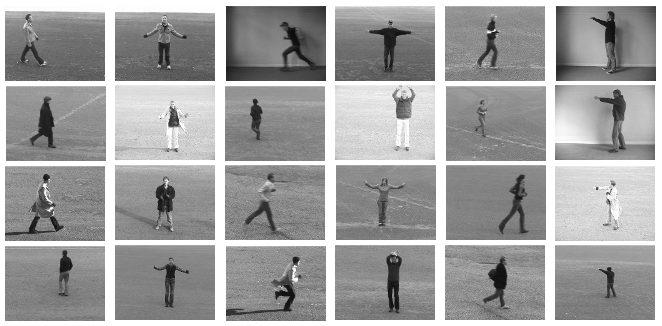
\includegraphics[scale=0.5]{img/ch2/KTH}
\caption[KTH Dataset]{Conjunto de Datos KTH, desarrolla seis actividades humanas ejecutadas por 25 actores en cuatro diferentes ambientes, facilitando 2391 acciones en 598 secuencias}
\label{fig:kth}
\end{figure}



El conjunto de datos Weizmann \cite {gorelick_actions_2007} (ver figura \ref{fig:weizmann}), fue construido para comprobar robustez de un método detección y clasificación de acciones humanas utilizando el concepto volumen espacio-tiempo. Consiste de 90 secuencias de baja resolución, diez acciones distintas ejecutadas por nueve actores en diferentes escenarios y imagen de fondo. Las imágenes son capturadas por una cámara estática localizada frente a estos actores. 

\begin{figure}[h!]
\centering
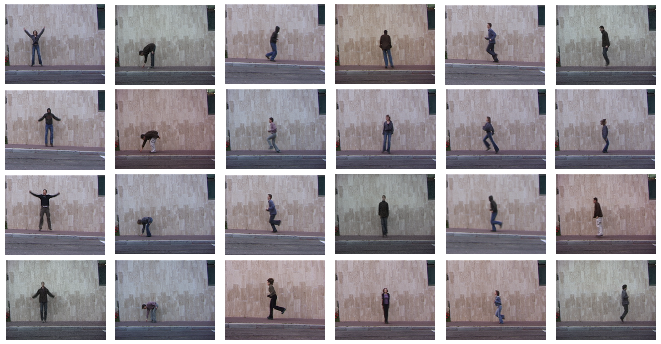
\includegraphics[scale=0.5]{img/ch2/Weizmann}
\caption[Weizmann Dataset]{Conjunto de Datos Weizmann consiste en diez acciones realizadas por nueve actores}
\label{fig:weizmann}
\end{figure}


MuHAVi \cite{singh_muhavi_2010} Es un conjunto de acciones humanas recolectados desde ocho ubicaciones diferentes (8 camaras), en un escenario irregular emulando iluminación nocturna de la calle. Contiene 17 clases diferentes de actividades, ejecutado por 14 actores (figura \ref{fig:muhavi}). INRIA XMAS \cite{weinland_free_2006} (figura \ref{fig:ixmas}) muy similar a MuHAVI \cite{singh_muhavi_2010}, se compone de 11 actividades cotidianas, por ejemplo, mirar la hora, darse vuelta, o caminar, entre otras. Cada acción es ejecutada en tres oportunidades por dies actores, cinco hombres y cinco mujeres. Una de las característica de este conjunto, se refiere que la posición y dirección de las actividades son realizadas en forma libre por los actores, de esta manera se logra que las actividades sean invariante a la vista (\textit{view-invariance}). 


\begin{figure}[h!]
\centering
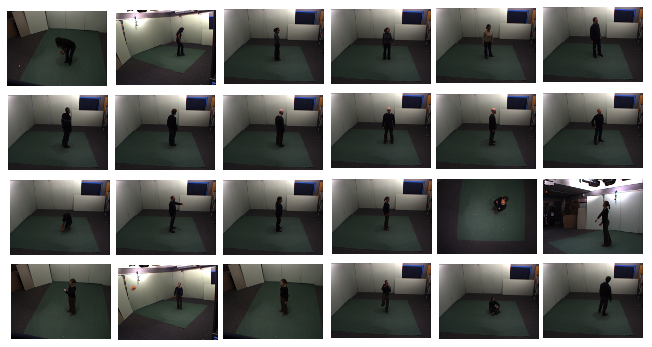
\includegraphics[scale=0.5]{img/ch2/ixmas}
\caption[IXMAS Dataset]{Conjunto de Datos IXMAS, es un ejemplo de 11 actividades cotidianas elaborada con diez actores}
\label{fig:ixmas}
\end{figure}

\begin{figure}[h!]
\centering
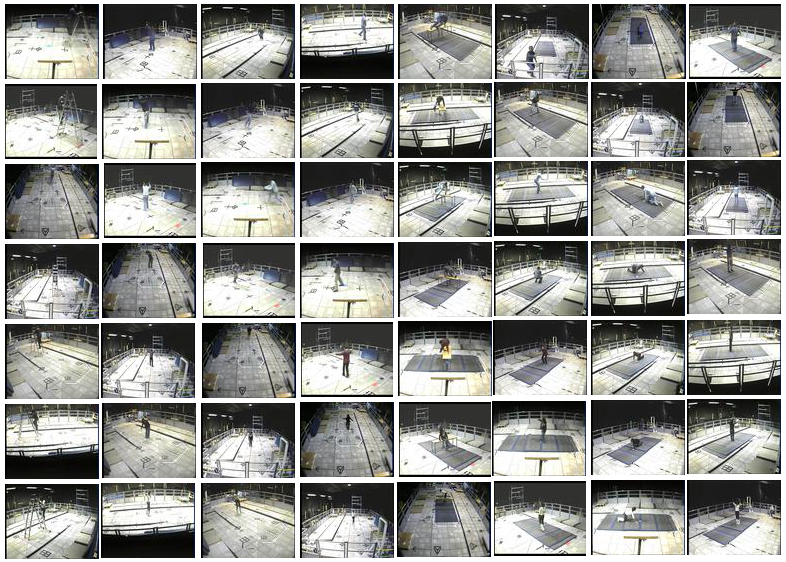
\includegraphics[scale=0.6]{img/ch2/MuHAVI}
\caption[MuHAVI Dataset]{Conjunto de Datos MuHAVI, son 7 actores desarrollando 17 acciones diferentes en un escenario simulando ilumanción nocturna.}
\label{fig:muhavi}
\end{figure}




